% !TeX program = xelatex
\documentclass[11pt,a4paper]{article}

% ============================================================
% Korean / Fonts
% Overleaf compiler: XeLaTeX
% ============================================================
\usepackage{kotex}
\usepackage{fontspec}

% ============================================================
% Mathematics
% ============================================================
\usepackage{amsmath,amssymb,bm,mathtools}

% ============================================================
% Page / Table
% ============================================================
\usepackage[
    left=25mm,
    right=25mm,
    top=25mm,
    bottom=25mm
]{geometry}
\usepackage{booktabs}
\usepackage{array}
\usepackage{enumitem}

\setlength{\parindent}{0pt}
\setlength{\parskip}{0.55em}

\title{\textbf{Gradient Descent와 Newton's Method}}
\author{}
\date{}

\usepackage{setspace}

\setstretch{1.3}

\begin{document}

\maketitle

% ============================================================
\section{최적화 문제}
% ============================================================

딥러닝에서 학습(training)은 주어진 loss function을 parameter에 대하여 최소화하는
최적화 문제로 이해할 수 있다. 먼저 1변수 함수의 간단한 최적화 문제를 생각하자.
\[
    \min_{x\in\mathbb{R}} f(x).
\]

$x^*$를 $f$의 최솟점이라고 하자. $f$가 미분 가능하면 최솟점에서
\[
    f'(x^*)=0
\]
이 성립한다. Gradient Descent와 Newton's method는 초기값 $x_0$에서 시작하여
반복적으로 새로운 점을 생성하고 $x^*$에 접근한다.

% ============================================================
\section{Gradient Descent}
% ============================================================

Gradient Descent(경사하강법)는 현재 위치에서 함수의 일차 미분값만을 이용한다.
1변수에서 $f'(x_k)$는 함수가 증가하는 방향을 나타내므로 그 반대 방향으로 이동한다.
\[
    \boxed{
    x_{k+1}=x_k-\alpha f'(x_k),
    \qquad \alpha>0
    }
\]

$\alpha$는 learning rate(학습률)이다. 이동 방향은 기울기가 결정하지만 실제 이동량은
기울기의 크기와 learning rate의 선택에 함께 의존한다.


% ============================================================
\section{Newton's Method}
% ============================================================

\begin{figure}[ht]
    \centering
    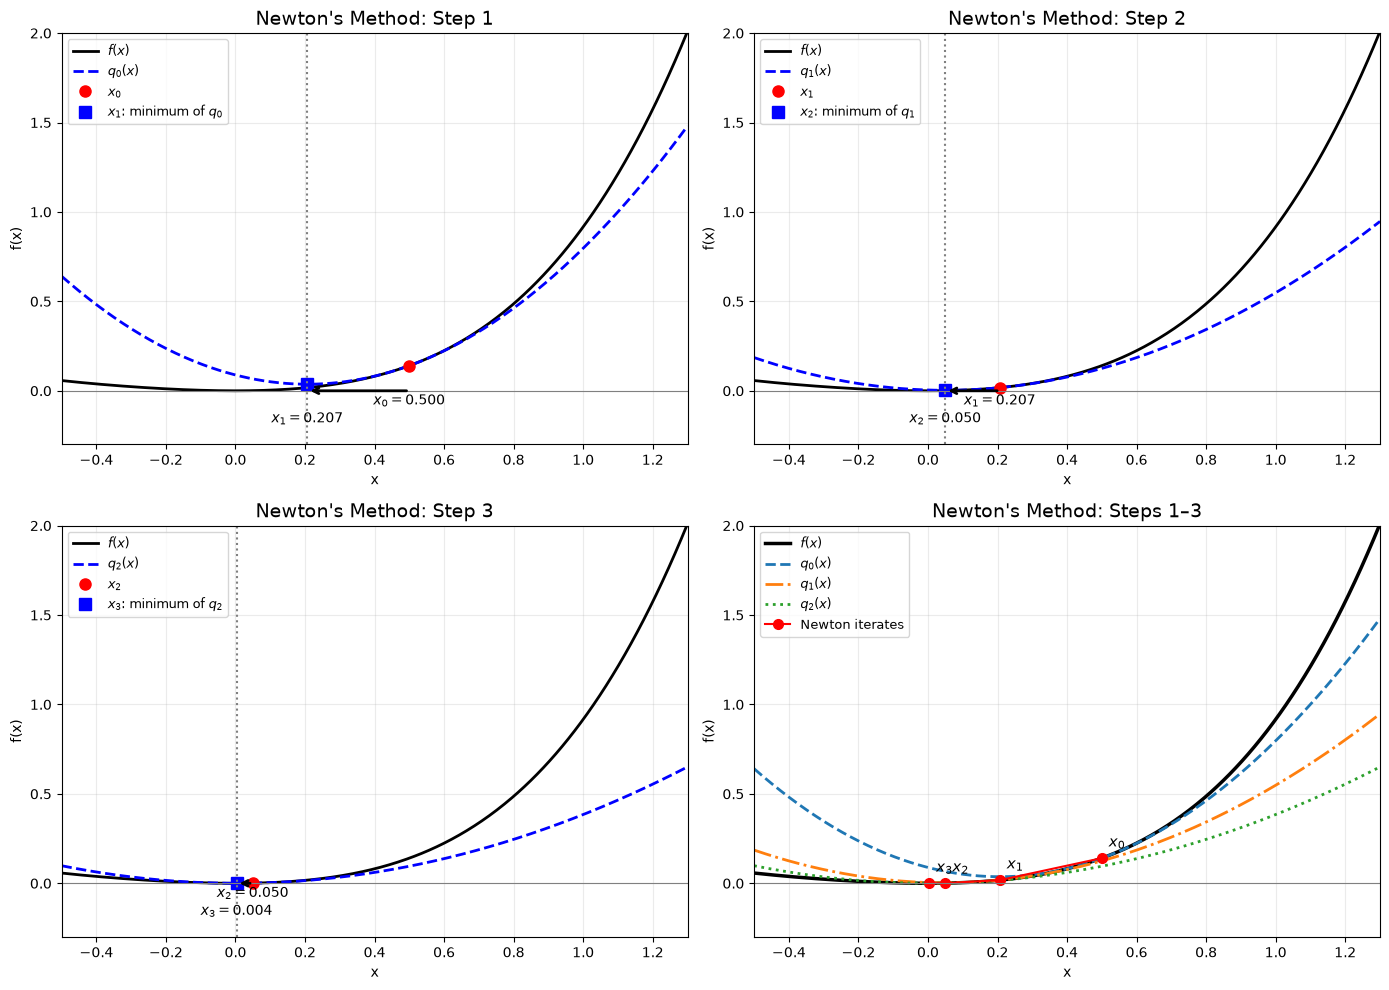
\includegraphics[width=0.9\textwidth]{../figures/newton_1variable.png}
    \caption{Newton's method는 현재점에서의 이차 근사함수의 최솟점을 다음 iterate로 선택한다.}
\end{figure}

Newton's method는 기울기뿐 아니라 곡률(curvature), 즉 이차 미분까지 이용한다.
현재점 $x_k$에서 $f$를 이차 Taylor 다항식으로 근사한다.

\[
    q_k(x)
    =
    f(x_k)
    +
    f'(x_k)(x-x_k)
    +
    \frac12 f''(x_k)(x-x_k)^2.
\]

$f''(x_k)>0$이면 $q_k$는 위로 열린 포물선이다. Newton's method는 이 이차
근사함수의 최솟점을 다음 iterate로 선택한다.
\[
q_k'(x)= f'(x_k)+f''(x_k)(x-x_k)=0
\quad\Longrightarrow\quad
x=x_k-\frac{f'(x_k)}{f''(x_k)}
=x_{k+1}.
\]


\[
    \boxed{
    x_{k+1}
    =
    x_k-\frac{f'(x_k)}{f''(x_k)}, \quad k=0,1,2,\ldots
    }
\]

따라서 Gradient Descent는 기울기와 미리 정한 learning rate를 사용하고,
Newton's method는 곡률을 이용하여 step의 크기까지 결정한다.


% ============================================================
\section{동일한 함수에서 3-step 비교}
% ============================================================

Newton's method의 일반적인 quadratic convergence가 실제로 나타나는 다음 함수를 사용하자.

\[
    f(x)
    =
    \frac12 x^2+\frac13 x^3+\frac14 x^4,
\]

\[
    f'(x)=x+x^2+x^3,
    \qquad
    f''(x)=1+2x+3x^2.
\]

$f'(x)=x(1+x+x^2)$이고 $1+x+x^2>0$이므로 유일한 stationary point는
$x^*=0$이다. 또한 $f''(0)=1>0$이므로 $x^*=0$은 최솟점이다.
두 방법 모두 $x_0=0.5$에서 시작한다.

\subsection{Gradient Descent: $\alpha=0.2$}

\[
\begin{aligned}
x_1
&=x_0-0.2f'(x_0)
 =0.500000-0.2(0.875000)
 =0.325000,\\
x_2
&=x_1-0.2f'(x_1)
 =0.325000-0.2(0.464953)
 =0.232009,\\
x_3
&=x_2-0.2f'(x_2)
 =0.232009-0.2(0.298326)
 =0.172344.
\end{aligned}
\]

따라서 세 번의 iteration은
\[
0.500000
\longrightarrow
0.325000
\longrightarrow
0.232009
\longrightarrow
0.172344.
\]

\subsection{Newton's Method}

\[
\begin{aligned}
x_1
&=x_0-\frac{0.875000}{2.750000}
 =0.181818,\\
x_2
&=x_1-\frac{0.220887}{1.462810}
 =0.030817,\\
x_3
&=x_2-\frac{0.031796}{1.064482}
 =0.000947.
\end{aligned}
\]

따라서 세 번의 iteration은
\[
0.500000
\longrightarrow
0.181818
\longrightarrow
0.030817
\longrightarrow
0.000947.
\]

\begin{center}
\begin{tabular}{ccc}
\toprule
$k$ & Gradient Descent & Newton's Method\\
\midrule
0 & 0.500000 & 0.500000\\
1 & 0.325000 & 0.181818\\
2 & 0.232009 & 0.030817\\
3 & 0.172344 & 0.000947\\
\bottomrule
\end{tabular}
\end{center}

3 step만 비교해도 이 예제에서는 Newton's method가 훨씬 빠르게 $x^*=0$에 접근한다. 
그러나 하나의 수치 예제만으로 일반적인 수렴 속도를 결론낼 수는 없다. 
일반적으로 gradient descent는 1차 수렴을, Newton’s method는 2차 수렴성을 갖는다고 알려져 있다. 
다음에서 대략적인 이유를 살펴보자.


% ============================================================
\section{수렴 차수 (Order of Convergence)}
% ============================================================

$k$번째 iterate의 오차(error)를 다음과 같이 정의하자.

\[
    e_k=x_k-x^*.
\]

수열 $x_k$가 $x^*$로 수렴한다고 하자. 충분히 큰 $k$에서 어떤 상수 $C>0$에 대하여

\[
    |e_{k+1}|
    \le C|e_k|^p
\]

가 성립하면 $p$를 수렴 차수(order of convergence)라고 한다.
$p=1$이고 $0<C<1$이면 linear convergence(선형 수렴),
$p=2$이면 quadratic convergence(이차 수렴)라고 한다.


% ============================================================
\section{Gradient Descent의 Linear Convergence}
% ============================================================

$f$가 $x^*$ 근방에서 두 번 연속 미분 가능하고 $x^*$가 strict local minimum이라고 하자.

\[
    f'(x^*)=0,
    \qquad
    f''(x^*)>0.
\]

또한 learning rate $\alpha$를 적절히 선택하여

\[
    |1-\alpha f''(x^*)|<1
\]

이고, $x_k$가 $x^*$에 충분히 가까운 영역에 있다고 하자.

Gradient Descent iteration은

\[
    x_{k+1}=x_k-\alpha f'(x_k),
    \qquad \alpha>0.
\]

양변에서 $x^*$를 빼면

\[
    e_{k+1}
    =
    e_k-\alpha f'(x_k).
\]

$f'$에 평균값 정리(Mean Value Theorem)를 적용하면 $x^*$와 $x_k$ 사이의
어떤 $\xi_k$가 존재하여

\[
    f'(x_k)-f'(x^*)
    =
    f''(\xi_k)(x_k-x^*)
\]

가 성립한다. $f'(x^*)=0$, $e_k=x_k-x^*$이므로

\[
    f'(x_k)=f''(\xi_k)e_k.
\]

따라서

\[
    \boxed{
    e_{k+1}
    =
    \left[1-\alpha f''(\xi_k)\right]e_k
    }
\]

를 얻는다. 이것은 평균값 정리로부터 얻은 정확한 관계이다.

$x_k\to x^*$이면 $\xi_k\to x^*$이고 $f''$의 연속성에 의해

\[
    \frac{e_{k+1}}{e_k}
    \longrightarrow
    1-\alpha f''(x^*).
\]

따라서 충분히 큰 $k$에서

\[
    |e_{k+1}|
    \approx
    C|e_k|,
    \qquad
    C=|1-\alpha f''(x^*)|<1
\]

가 되어 Gradient Descent는 국소적으로 linear convergence를 보인다.
Taylor 전개를 이용하면 같은 사실을

\[
    e_{k+1}
    =
    \left[1-\alpha f''(x^*)\right]e_k
    +
    O(e_k^2)
\]

로 쓸 수 있다. 핵심은 leading error term이 $e_k$에 비례하여 남아 있다는 점이다.


% ============================================================
\section{Newton's Method의 Quadratic Convergence}
% ============================================================

$f$가 $x^*$ 근방에서 세 번 연속 미분 가능하고
\[
    f'(x^*)=0,
    \qquad
    f''(x^*)\neq 0
\]
이라고 하자. 초기값이 $x^*$에 충분히 가까워 모든 iterate에서
$f''(x_k)\neq0$이라고 가정한다.

Newton iteration은
\[
    x_{k+1}
    =
    x_k-\frac{f'(x_k)}{f''(x_k)}.
\]

$f'(x^*)$를 $x_k$를 중심으로 Taylor 전개한다. Taylor 정리에 의해
$x_k$와 $x^*$ 사이의 어떤 $\xi_k$가 존재하여
\[
    f'(x^*)
    =
    f'(x_k)
    +
    f''(x_k)(x^*-x_k)
    +
    \frac12 f'''(\xi_k)(x^*-x_k)^2.
\]

$f'(x^*)=0$, $x^*-x_k=-e_k$를 대입하면
\[
    0
    =
    f'(x_k)
    -
    f''(x_k)e_k
    +
    \frac12 f'''(\xi_k)e_k^2.
\]

따라서
\[
    f'(x_k)
    =
    f''(x_k)e_k
    -
    \frac12 f'''(\xi_k)e_k^2.
\]

Newton iteration에서 $x^*$를 빼고 위 식을 대입하면 일차 오차항이 정확히 소거되어
\[
\begin{aligned}
e_{k+1}
&=
e_k-\frac{f'(x_k)}{f''(x_k)}=
\frac{f'''(\xi_k)}{2f''(x_k)}e_k^2.
\end{aligned}
\]

즉,
\[
    \boxed{
    e_{k+1}
    =
    \frac{f'''(\xi_k)}{2f''(x_k)}e_k^2
    }.
\]

$x_k\to x^*$이면 $\xi_k\to x^*$이므로, $f'''(x^*)\neq0$인 일반적인 경우

\[
    \frac{e_{k+1}}{e_k^2}
    \longrightarrow
    \frac{f'''(x^*)}{2f''(x^*)}.
\]

따라서 충분히 큰 $k$에서 어떤 $C>0$에 대하여

\[
    |e_{k+1}|
    \le
    C|e_k|^2
\]

가 성립한다. 이것이 Newton's method의 local quadratic convergence이다.
핵심은 곡률 정보를 이용하면서 일차 error term이 소거된다는 점이다.

\[
    \boxed{
    \text{Gradient Descent: }e_{k+1}=O(e_k),
    \qquad
    \text{Newton's Method: }e_{k+1}=O(e_k^2)
    }
\]

% ============================================================
\section{위 예제에서 Quadratic Convergence의 수치적 확인}
% ============================================================

선택한 함수에서는 $f''(0)=1$, $f'''(0)=2$이므로
Newton 수렴식의 점근적 상수는
\[
\frac{f'''(0)}{2f''(0)}
=
\frac{2}{2\cdot 1}
=
1
\]
이다. 따라서 $x_k$가 $0$에 충분히 가까워지면
\[
|e_{k+1}| \approx |e_k|^2
\]
가 나타나야 한다. $x^*=0$이므로 $e_k=x_k$이다.

\[
\frac{|e_1|}{|e_0|^2}=0.7273,
\qquad
\frac{|e_2|}{|e_1|^2}=0.9322,
\qquad
\frac{|e_3|}{|e_2|^2}=0.9973.
\]

이 비율이 $1$에 가까워지는 것이 이 예제에서
Newton's method의 quadratic convergence를 수치적으로 확인하는 방법이다.

% ============================================================
\section{다변수 문제로의 확장 (Multivariable Optimization)}
% ============================================================

지금까지는 $f:\mathbb{R}\to\mathbb{R}$인 1변수 함수에서 Gradient Descent와
Newton's method를 살펴보았다. 딥러닝에서 실제로 최소화하는 loss function은
수많은 parameter를 가지므로, 이제 이를 $n$개의 변수를 갖는 함수로 확장한다.
다변수에서는 1차 미분은 \textbf{gradient}, 2차 미분은
\textbf{Hessian matrix}로 일반화된다. 수렴성에 대한 엄밀한 증명은 생략하고,
각 알고리즘이 어떤 정보를 사용하며 어떻게 계산되는지에 초점을 맞춘다.

\subsection{다변수 최적화 문제}

다음의 unconstrained optimization problem을 생각하자.

\[
    \min_{\mathbf{x}\in\mathbb{R}^n} f(\mathbf{x}),
    \qquad
    \mathbf{x}
    =
    \begin{bmatrix}
    x_1\\
    x_2\\
    \vdots\\
    x_n
    \end{bmatrix},
    \qquad
    f:\mathbb{R}^n\to\mathbb{R}.
\]

여기서 $\mathbf{x}$는 최적화해야 할 parameter vector이다.
딥러닝에서는 $\mathbf{x}$ 대신 보통 $\boldsymbol{\theta}$를 사용하여
network의 모든 weight와 bias를 하나의 parameter vector로 생각한다.

미분 가능한 함수 $f$가 $\mathbf{x}^*$에서 local minimum을 가지면
필요한 일차 조건(first-order necessary condition)은
\[
    \nabla f(\mathbf{x}^*)=\mathbf{0}
\]
이다. 그러나 다변수에서도 $\nabla f=\mathbf{0}$이라는 조건만으로
local minimum이 보장되는 것은 아니다. 그 점이 minimum인지 maximum인지
saddle point인지 판단하려면 2차 미분 정보인 Hessian을 살펴보아야 한다.

\subsection{Gradient: 다변수에서의 일차 미분}

$f(\mathbf{x})=f(x_1,\ldots,x_n)$의 gradient는 각 변수에 대한 편미분을
모은 column vector이다.

\[
    \nabla f(\mathbf{x})
    =
    \begin{bmatrix}
    \dfrac{\partial f}{\partial x_1}\\[2mm]
    \dfrac{\partial f}{\partial x_2}\\
    \vdots\\
    \dfrac{\partial f}{\partial x_n}
    \end{bmatrix}.
\]

현재점 $\mathbf{x}$에서 unit vector $\mathbf{v}$ 방향으로의
directional derivative는
\[
    D_{\mathbf{v}}f(\mathbf{x})
    =
    \nabla f(\mathbf{x})^T\mathbf{v}.
\]

$\|\mathbf{v}\|=1$이면 Cauchy--Schwarz inequality에 의해
\[
    -\|\nabla f(\mathbf{x})\|
    \le
    \nabla f(\mathbf{x})^T\mathbf{v}
    \le
    \|\nabla f(\mathbf{x})\|.
\]

이때, 왼쪽 등호는 $\mathbf{v}=-\frac{\nabla f(\mathbf{x})}{\|\nabla f(\mathbf{x})\|}$일 때 성립하고 오른쪽 등호는
 $\mathbf{v}=\frac{\nabla f(\mathbf{x})}{\|\nabla f(\mathbf{x})\|}$일 때 성립한다. 따라서 $\nabla f(\mathbf{x})$는 함수값이 가장 빠르게 증가하는 방향이고,
$-\nabla f(\mathbf{x})$는 가장 빠르게 감소하는 방향이다.


\subsection{다변수 Gradient Descent}

현재점 $\mathbf{x}_k$에서 $f$ 를 가장 빠르게 감소시키는 방향은 $\nabla f(\mathbf{x}_k)$이고, 따라서 Gradient Descent는
$-\nabla f(\mathbf{x}_k)$로 이동한다.

\[
    \boxed{
    \mathbf{x}_{k+1}
    =
    \mathbf{x}_k-\alpha\nabla f(\mathbf{x}_k)
    }
\]

여기서 $\alpha>0$는 learning rate이다. 각 coordinate로 쓰면

\[
    x_{i,k+1}
    =
    x_{i,k}
    -
    \alpha
    \frac{\partial f}{\partial x_i}(\mathbf{x}_k),
    \qquad
    i=1,\ldots,n.
\]

따라서 하나의 iteration은 다음과 같다.

\begin{enumerate}[leftmargin=2.5em]
    \item 현재 parameter $\mathbf{x}_k$에서
    gradient $\mathbf{g}_k=\nabla f(\mathbf{x}_k)$를 계산한다.
    \item descent direction $-\mathbf{g}_k$를 정한다.
    \item learning rate $\alpha$만큼 이동하여
    $\mathbf{x}_{k+1}=\mathbf{x}_k-\alpha\mathbf{g}_k$를 얻는다.
    \item stopping criterion을 만족할 때까지 반복한다.
\end{enumerate}

Gradient는 이동 \textbf{방향}뿐 아니라 그 크기에도 영향을 주며,
실제 step length는

\[
    \|\mathbf{x}_{k+1}-\mathbf{x}_k\|
    =
    \alpha\|\nabla f(\mathbf{x}_k)\|
\]

이다. 

2차원에서 level curve
\[
f(x_1,x_2)=c
\]
를 생각하자. 이 곡선을
\[
\mathbf{c}(t)=(x_1(t),x_2(t))
\]
로 매개화하면, level curve 위에서는 항상
\[
f(\mathbf{c}(t))=c
\]
이므로 양변을 $t$에 대해 미분하여
\[
\frac{d}{dt}f(\mathbf{c}(t))
=
\nabla f(\mathbf{c}(t))^T\mathbf{x}'(t)
=0
\]
을 얻는다. 여기서 $\mathbf{c}'(t)$는 level curve의 접선 방향(tangent
direction)이므로,
\[
\nabla f(\mathbf{c}(t))\perp \mathbf{c}'(t).
\]
따라서 gradient $\nabla f$는 level curve에 수직이다.
2차원에서 level curve $f(x_1,x_2)=c$를 생각하면 gradient는 그 level curve에
수직이다. 


\subsection{Hessian Matrix: 다변수에서의 이차 미분}

1변수에서 곡률 정보를 $f''(x)$가 나타냈다면, 다변수에서는 모든
2차 편미분을 모은 Hessian matrix가 그 역할을 한다.

\[
H(\mathbf{x})
=
\nabla^2 f(\mathbf{x})
=
\begin{bmatrix}
\dfrac{\partial^2 f}{\partial x_1^2}
&
\dfrac{\partial^2 f}{\partial x_1\partial x_2}
&
\cdots
&
\dfrac{\partial^2 f}{\partial x_1\partial x_n}
\\[2mm]
\dfrac{\partial^2 f}{\partial x_2\partial x_1}
&
\dfrac{\partial^2 f}{\partial x_2^2}
&
\cdots
&
\dfrac{\partial^2 f}{\partial x_2\partial x_n}
\\
\vdots & \vdots & \ddots & \vdots
\\
\dfrac{\partial^2 f}{\partial x_n\partial x_1}
&
\dfrac{\partial^2 f}{\partial x_n\partial x_2}
&
\cdots
&
\dfrac{\partial^2 f}{\partial x_n^2}
\end{bmatrix}.
\]

$f$의 2차 편미분이 연속이면 mixed partial derivatives가 같으므로

\[
    \frac{\partial^2f}{\partial x_i\partial x_j}
    =
    \frac{\partial^2f}{\partial x_j\partial x_i}.
\]

따라서 Hessian은 symmetric matrix이다.

특히 2변수 함수 $f(x,y)$에서는

\[
    H(x,y)
    =
    \begin{bmatrix}
    f_{xx} & f_{xy}\\
    f_{yx} & f_{yy}
    \end{bmatrix}
    =
    \begin{bmatrix}
    f_{xx} & f_{xy}\\
    f_{xy} & f_{yy}
    \end{bmatrix}.
\]

Hessian은 단순히 각 coordinate 방향의 곡률만을 담는 것이 아니다.
임의의 unit direction $\mathbf{v}$에 대한 이차 방향미분
(second directional derivative)은

\[
    D_{\mathbf{v}}^2f(\mathbf{x})
    =
    \mathbf{v}^T H(\mathbf{x})\mathbf{v}
\]

이므로, Hessian은 모든 방향에 대한 local curvature를 동시에 담고 있다.

\subsection{Hessian과 local geometry}

Stationary point $\mathbf{x}^*$에서
\[
    \nabla f(\mathbf{x}^*)=\mathbf{0}
\]
이라고 하자. Hessian의 eigenvalue를 보면 그 점 근방의 geometry를 이해할 수 있다.

\begin{itemize}[leftmargin=2em]
    \item 모든 eigenvalue가 양수이면
    $H(\mathbf{x}^*)\succ0$이고, $\mathbf{x}^*$는 strict local minimum이다.

    \item 모든 eigenvalue가 음수이면
    $H(\mathbf{x}^*)\prec0$이고, $\mathbf{x}^*$는 strict local maximum이다.

    \item 양수와 음수 eigenvalue가 모두 있으면 Hessian은 indefinite이고,
    $\mathbf{x}^*$는 saddle point이다.

    \item zero eigenvalue가 있으면 이 2차 정보만으로는 결론을 내리지 못할 수 있다.
\end{itemize}

즉 1변수에서 $f''(x^*)>0$이면 위로 열린 포물선 모양이 되는 것처럼,
다변수에서 $H(\mathbf{x}^*)\succ0$이면 모든 방향으로 위로 휘어진
bowl-shaped local geometry를 갖는다.

\subsection{다변수 Taylor Expansion}

1변수에서 Newton's method를 유도할 때 사용한 quadratic Taylor polynomial을
다변수로 확장해 보자. 현재점 $\mathbf{x}_k$에서 작은 displacement
$\mathbf{p}$만큼 이동한 점을

\[
    \mathbf{x}=\mathbf{x}_k+\mathbf{p}
\]

라고 하자. $f$의 2차 Taylor approximation은

\[
    \boxed{
    q_k(\mathbf{p})
    =
    f(\mathbf{x}_k)
    +
    \nabla f(\mathbf{x}_k)^T\mathbf{p}
    +
    \frac12\mathbf{p}^T
    H(\mathbf{x}_k)\mathbf{p}
    }
\]

이다. 따라서

\[
    f(\mathbf{x}_k+\mathbf{p})
    \approx
    q_k(\mathbf{p}).
\]

각 항의 의미는 다음과 같다.

\[
\underbrace{f(\mathbf{x}_k)}_{\text{현재 함수값}}
+
\underbrace{\nabla f(\mathbf{x}_k)^T\mathbf{p}}_{\text{1차 변화: slope}}
+
\underbrace{\frac12\mathbf{p}^T H(\mathbf{x}_k)\mathbf{p}}_{\text{2차 변화: curvature}}.
\]

1변수에서 $p=x-x_k$라고 두면 위 식은 정확히

\[
    f(x_k+p)
    \approx
    f(x_k)+f'(x_k)p+\frac12f''(x_k)p^2
\]

로 돌아간다. 즉 gradient와 Hessian은 각각 1변수의 $f'$와 $f''$를
자연스럽게 일반화한 것이다.


\subsection{다변수 Newton's Method의 유도}

Newton's method는 현재점에서의 quadratic approximation $q_k$ 자체를
최소화하여 다음 step을 결정한다. 간단히

\[
    \mathbf{g}_k=\nabla f(\mathbf{x}_k),
    \qquad
    H_k=H(\mathbf{x}_k)
\]

라고 쓰면

\[
    q_k(\mathbf{p})
    =
    f(\mathbf{x}_k)
    +
    \mathbf{g}_k^T\mathbf{p}
    +
    \frac12\mathbf{p}^T H_k\mathbf{p}.
\]

$H_k$가 symmetric이므로 $\mathbf{p}$에 대한 gradient는

\[
    \nabla_{\mathbf{p}}q_k(\mathbf{p})
    =
    \mathbf{g}_k+H_k\mathbf{p}.
\]

quadratic approximation의 minimizer에서는 이 gradient가 zero가 되어야 하므로

\[
    \mathbf{g}_k+H_k\mathbf{p}_k=\mathbf{0}.
\]

따라서 Newton step $\mathbf{p}_k$는 다음 linear system의 해이다.

\[
    \boxed{
    H_k\mathbf{p}_k=-\mathbf{g}_k
    }
\]

$H_k$가 invertible이면 형식적으로

\[
    \mathbf{p}_k=-H_k^{-1}\mathbf{g}_k
\]

이고, 따라서

\[
    \boxed{
    \mathbf{x}_{k+1}
    =
    \mathbf{x}_k
    -
    H(\mathbf{x}_k)^{-1}
    \nabla f(\mathbf{x}_k)
    }
\]

을 얻는다.

그러나 실제 numerical computation에서는 $H_k^{-1}$을 직접 계산하는 것이 아니라

\[
    H_k\mathbf{p}_k=-\mathbf{g}_k
\]

라는 linear system을 풀어 $\mathbf{p}_k$를 구하는 것이 일반적이다.
Matrix inverse를 명시적으로 계산하는 것보다 이 방식이 더 효율적이고
수치적으로도 안정적이다.

\subsection{Gradient Descent와 Newton Direction의 차이}

두 방법의 step을 비교하면

\[
    \mathbf{p}_k^{\mathrm{GD}}
    =
    -\alpha\mathbf{g}_k,
    \qquad
    \mathbf{p}_k^{\mathrm{Newton}}
    =
    -H_k^{-1}\mathbf{g}_k.
\]

Gradient Descent에서는 하나의 scalar $\alpha$가 모든 방향의 step size를 조절한다.
반면 Newton's method에서는 $H_k^{-1}$가 gradient를 방향별 curvature에 따라 변형한다.

Hessian의 eigendecomposition을

\[
    H_k=Q\Lambda Q^T,
    \qquad
    \Lambda
    =
    \operatorname{diag}(\lambda_1,\ldots,\lambda_n)
\]

라고 하면

\[
    H_k^{-1}
    =
    Q\Lambda^{-1}Q^T.
\]

따라서 Newton step은 Hessian의 eigenvector 방향으로 gradient를 분해한 뒤,
각 성분을 $1/\lambda_i$만큼 scaling한다. 곡률 $\lambda_i$가 큰 방향에서는
작은 step을, 곡률이 작은 방향에서는 상대적으로 큰 step을 취한다.
즉 Newton's method는 local geometry에 맞추어 방향과 step size를 동시에 조정한다.

이 때문에 길고 좁은 valley처럼 방향에 따라 curvature가 크게 다른 문제에서
Gradient Descent는 zig-zagging할 수 있지만, Newton's method는 curvature를
보정하여 훨씬 직접적인 step을 만들 수 있다.

\subsection{2변수 Quadratic Function에서의 예}

다음의 quadratic function을 생각하자.

\[
    f(x,y)
    =
    \frac12
    \begin{bmatrix}
    x & y
    \end{bmatrix}
    \begin{bmatrix}
    a & c\\
    c & b
    \end{bmatrix}
    \begin{bmatrix}
    x\\y
    \end{bmatrix},
\]

또는

\[
    f(\mathbf{x})
    =
    \frac12\mathbf{x}^T A\mathbf{x},
    \qquad
    A=A^T\succ0.
\]

이때

\[
    \nabla f(\mathbf{x})=A\mathbf{x},
    \qquad
    H(\mathbf{x})=A.
\]

따라서 Gradient Descent는

\[
    \mathbf{x}_{k+1}
    =
    \mathbf{x}_k-\alpha A\mathbf{x}_k
\]

이고, Newton's method는

\[
\begin{aligned}
    \mathbf{x}_{k+1}
    &=
    \mathbf{x}_k-A^{-1}A\mathbf{x}_k\\
    &=\mathbf{0}.
\end{aligned}
\]

즉 $A\succ0$인 정확한 quadratic function에서는 Newton's method가
초기값과 관계없이 한 번의 iteration으로 minimizer $\mathbf{x}^*=\mathbf{0}$에
도달한다.

일반적인 nonlinear function에서는 함수가 정확한 quadratic이 아니므로
매 iteration마다 새로운 Hessian을 계산하고 local quadratic model을 다시 만든다.


\subsection{예제}
다음의 이차함수를 생각하자.
\[
f(x_1,x_2)
=
3(x_1-6)^2+(x_2-5)^2.
\]
이 함수는 $ \mathbf{x}^*=(6,5)$에서 유일한 최솟값을 가지며,
\[
f(6,5)=0
\]
이다. 함수의 gradient는
\[
\nabla f(x_1,x_2)
=
\begin{bmatrix}
6(x_1-6)\\
2(x_2-5)
\end{bmatrix}
\]
로 주어진다.

따라서 Gradient Descent iteration은
\[
\mathbf{x}_{k+1}
=
\mathbf{x}_k-\alpha\nabla f(\mathbf{x}_k)
\]
이고, 각 성분으로 표현하면
\[
\begin{aligned}
x_{1,k+1}
&=
x_{1,k}-6\alpha(x_{1,k}-6),\\
x_{2,k+1}
&=
x_{2,k}-2\alpha(x_{2,k}-5).
\end{aligned}
\]

초깃값을
\[
\mathbf{x}_0=(1,1)
\]
로 선택하고 learning rate를 $\alpha=0.05$로 설정하여
Gradient Descent를 수행한다.


\begin{figure}
\centering
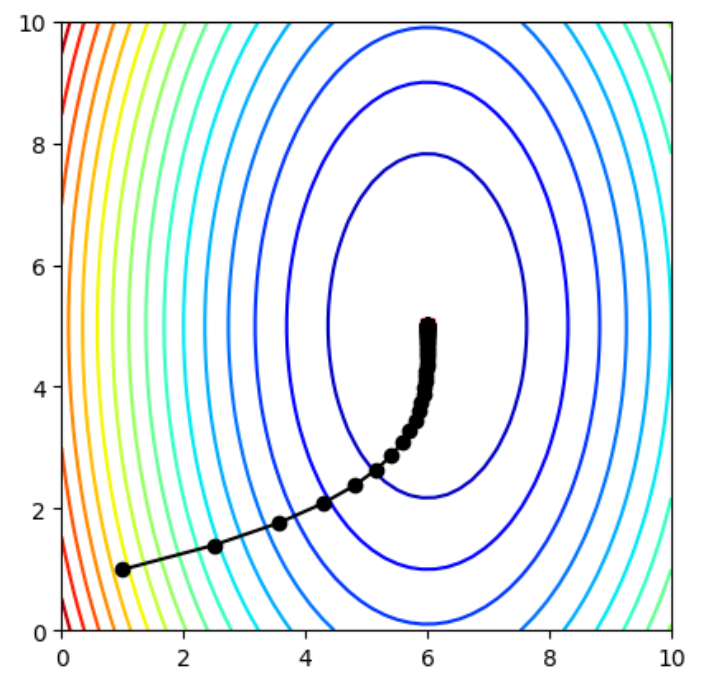
\includegraphics[width=0.48\textwidth]{../figures/gradient_descent_2variables_levelset.png}
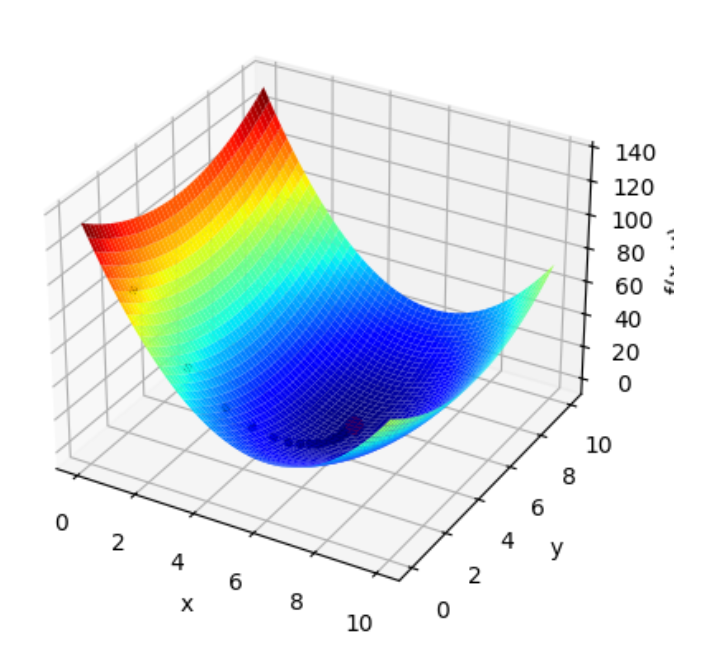
\includegraphics[width=0.48\textwidth]{../figures/gradient_descent_2variables_surface.png}
\caption{Gradient Descent의 이동 경로. 왼쪽 그림은 level curve 위에서의 이동 경로를 보여주고, 오른쪽 그림은 3D surface plot에서의 이동 경로를 보여준다.}
\end{figure}


이 함수의 level curve는
\[
3(x_1-6)^2+(x_2-5)^2=c
\]
이므로 $(6,5)$를 중심으로 하는 타원(ellipse)이다.
Gradient $\nabla f$는 각 점에서 이 level curve에 수직이며,
$-\nabla f$는 그 점에서 함수값을 가장 빠르게 감소시키는 방향을 나타낸다.
따라서 Gradient Descent는 매 iteration마다 현재 위치에서
$-\nabla f$ 방향으로 이동하면서 최솟점 $(6,5)$에 접근한다.

특히 이 예제에서는 $x_1$ 방향과 $x_2$ 방향의 curvature가 서로 다르다.
Hessian은
\[
H=
\begin{bmatrix}
6&0\\
0&2
\end{bmatrix}
\]
이므로 $x_1$ 방향의 curvature가 $x_2$ 방향보다 크다.
따라서 등고선은 원이 아니라 타원 형태를 가지며,
Gradient Descent의 이동 경로 역시 최솟점까지의 직선 경로가 아니라
각 위치에서의 local steepest descent direction을 따라 결정된다.

같은 문제에 Newton's method를 적용해 보자. 함수
\[
f(x_1,x_2)=3(x_1-6)^2+(x_2-5)^2
\]
의 gradient와 Hessian은 각각
\[
\nabla f(x_1,x_2)
=
\begin{bmatrix}
6(x_1-6)\\
2(x_2-5)
\end{bmatrix},
\qquad
H=
\begin{bmatrix}
6&0\\
0&2
\end{bmatrix}.
\]

Newton's method는
\[
\mathbf{x}_{k+1}
=
\mathbf{x}_k-H^{-1}\nabla f(\mathbf{x}_k)
\]
로 주어진다. 이 예제에서는
\[
H^{-1}
=
\begin{bmatrix}
1/6&0\\
0&1/2
\end{bmatrix}
\]
이므로
\[
H^{-1}\nabla f(\mathbf{x}_k)
=
\begin{bmatrix}
x_{1,k}-6\\
x_{2,k}-5
\end{bmatrix}.
\]

따라서
\[
\mathbf{x}_{k+1}
=
\begin{bmatrix}
x_{1,k}\\
x_{2,k}
\end{bmatrix}
-
\begin{bmatrix}
x_{1,k}-6\\
x_{2,k}-5
\end{bmatrix}
=
\begin{bmatrix}
6\\
5
\end{bmatrix} = \mathbf{x}^*.
\]

즉, 어떠한 초깃값 $\mathbf{x}_0$에서 시작하더라도 Newton's method는
이 문제에서는 단 한 번의 iteration으로 정확한 최솟점 $(6,5)$에 도달한다.

\subsubsection{계산비용의 관점}

Gradient Descent는 각 iteration에서 gradient
\[
\nabla f(\mathbf{x}_k)
\]
만 계산하면 된다. 반면 Newton's method는 gradient뿐만 아니라 Hessian
\[
H(\mathbf{x}_k)=\nabla^2 f(\mathbf{x}_k)
\]
을 계산해야 하며, Newton direction을 구하기 위해
\[
H(\mathbf{x}_k)\mathbf{p}_k
=
-\nabla f(\mathbf{x}_k)
\]
라는 선형시스템을 풀어야 한다.

변수의 개수가 $n$개라면 Hessian은 $n\times n$ 행렬이다.
따라서 Hessian을 직접 저장하는 데에는 대략
\[
O(n^2)
\]
의 memory가 필요하고, 일반적인 dense linear system을 푸는 데에는
대략
\[
O(n^3)
\]
의 계산비용이 필요하다.

예를 들어 neural network가 $10^6$개의 parameters를 가진다면 Hessian은
\[
10^6\times 10^6=10^{12}
\]
개의 성분을 가진다. 각 성분을 32-bit floating point number로
저장한다고 해도 필요한 memory는 대략
\[
4\times 10^{12}\text{ bytes}\approx 4\text{ TB}
\]
가 된다. 따라서 대규모 neural network에서 Hessian을 직접 구성하여
Newton's method를 적용하는 것은 현실적으로 매우 어렵다.

그러나 Newton's method가 사용하는 \emph{curvature information} 자체는
매우 유용하다. 이를 실제 Hessian을 계산하지 않고 근사적으로 이용하는
방법이 \textbf{Quasi-Newton method}이다.

(참고) 두 successive iterations에서
\[
\mathbf{s}_k
=
\boldsymbol{\theta}_{k+1}-\boldsymbol{\theta}_k,
\qquad
\mathbf{y}_k
=
\nabla L(\boldsymbol{\theta}_{k+1})
-
\nabla L(\boldsymbol{\theta}_k)
\]
라고 하면, gradient의 Taylor expansion으로부터
\[
\mathbf{y}_k
\approx
H_k\mathbf{s}_k
\]
를 얻는다. 따라서 parameter와 gradient의 변화만을 이용하여
Hessian의 curvature information을 근사할 수 있다.

대표적인 Quasi-Newton method가 \textbf{BFGS}이며,
\textbf{L-BFGS (Limited-memory BFGS)}는 전체 Hessian 근사행렬을
저장하는 대신 최근의 몇 개의
$(\mathbf{s}_k,\mathbf{y}_k)$ 정보만을 저장하여 memory 사용량을
크게 줄인 방법이다.

즉, L-BFGS는 Newton's method의 curvature information을 활용하면서도
대규모 문제에서 Hessian을 직접 계산하고 저장해야 하는 부담을
줄이기 위한 Quasi-Newton method라고 볼 수 있다.


% ============================================================
\section{딥러닝과의 연결}

Neural network의 학습은 network parameters
$\boldsymbol{\theta}$에 대한 loss function
\[
L(\boldsymbol{\theta})
\]
을 최소화하는 optimization problem이다.

앞에서 살펴본 Newton's method는 Hessian을 이용하여 curvature information을
반영하므로 빠른 local convergence를 가질 수 있지만, 대규모 neural
network에서는 Hessian을 직접 계산하고 저장하는 비용이 너무 크다.
또한 neural network의 loss function은 일반적으로 nonconvex이므로
Newton's method를 그대로 적용하기에도 여러 어려움이 있다.

따라서 neural network의 초기 학습에서는 일반적으로 Hessian을 필요로 하지
않는 \textbf{first-order methods}를 사용한다. 대표적인 방법으로
\[
\text{SGD},\qquad
\text{Momentum},\qquad
\text{Adam}
\]
등이 있다. 이러한 방법들은 gradient information만을 이용하므로
대규모 parameter를 가지는 neural network의 학습에 적합하다.

한편 optimization이 진행되어 loss가 충분히 감소하고 parameters가
어느 정도 좋은 영역에 도달한 후에는, 필요에 따라 curvature information을
근사적으로 사용하는 Quasi-Newton method를 이용하여 보다 정밀한
local optimization을 수행할 수 있다.

대표적인 예가
\[
\boxed{
\text{Adam}
\quad\longrightarrow\quad
\text{L-BFGS}
}
\]
와 같은 optimization strategy이다.

즉, 초기에는 Adam과 같은 Gradient Descent 기반의 first-order method를
사용하여 parameter space를 안정적으로 탐색하고, 어느 정도 수렴성이
나타난 이후에는 L-BFGS와 같은 Quasi-Newton method를 사용하여
local curvature information을 활용하면서 보다 정밀한 수렴을
시도할 수 있다.

이러한 전략은 모든 deep learning 문제에서 반드시 사용되는 것은 아니지만,
특히 full-batch 또는 deterministic optimization의 성격이 강한 문제에서
유용할 수 있다. 대표적으로
\textbf{Physics-Informed Neural Networks (PINNs)}에서는
\[
\text{Adam} \;\longrightarrow\; \text{L-BFGS}
\]
조합이 널리 사용된다.

따라서 지금까지 살펴본 optimization methods의 관계를 다음과 같이
생각할 수 있다:
\[
\boxed{
\text{Gradient Descent}
\;\longrightarrow\;
\text{SGD / Momentum / Adam}
\;\longrightarrow\;
\text{BFGS / L-BFGS}
}
\]
여기서 앞의 방법들은 gradient를 기반으로 하는 first-order methods이고,
BFGS와 L-BFGS는 Newton's method의 curvature information을
근사적으로 이용하는 Quasi-Newton methods이다.
\end{document}
